\chapter{The simulator}
\label{ch:parallel-simulator}

\section{Decomposition}

To parallelize the simulation, the process must be decomposed in parts that can 
be executed in parallel and several decompositions are known.
%
One of the most common technique found in particle-in-cell codes, is the 
\textit{domain decomposition}---the physical space is divided into sections of 
similar size and the fields are assigned to different computing units. The main 
drawback of this technique is the risk of unbalanced load, as some regions of 
space may contain a large amount or even all the particles.

Another approach called \textit{particle decomposition} consists in the division 
of the particles into groups, where each processor maintains a copy of the 
fields of the whole space.  The problem of this method is the limitation of 
scalability, as the number of grid points used in the fields is limited by the 
memory of one computing element.

Additionally, the Fourier transform needed by the MFT solver is implemented 
using the FFTW library and the parallelization design provided by the library 
introduces a constraint in the distribution of the fields: they need to be 
broken into slices in the Y dimension, resulting in contiguous blocks of 
elements in X. Consequently, the domain decomposition is the chosen technique 
for the simulator.

\begin{figure}[ht]%{{{
\centering
\begin{tikzpicture}
\begin{scope}[
		x=1cm,
		y=1cm,
		yshift=0,
		every node/.append style={
			yslant=0.5,xslant=-1},
		yslant=0.5,
		xslant=-1
	]
	% opacity to prevent graphical interference
	\draw[step=1.5/8, black!20!white, thin] (0,0) grid (6,6); %defining grids
	%\draw[step=1.5, black] (0,0) grid (6,6);
	\draw[xstep=1.5, ystep=6, black, very thick] (0,0) grid (6,6);
	%\draw[dashed, xstep=6, ystep=1.5, black] (0,0) grid (6,6);
	\fill[fill=black,fill opacity=0.1] (0,0) rectangle (1.5,6);
	\coordinate (a0) at (4.5, 0);
	\coordinate (a1) at (6, 0);
	\coordinate (a2) at (4.5, 1.5);
	\coordinate (a3) at (6, 1.5);

	\coordinate (b) at (0,3);

\end{scope}
\begin{scope}[
		x=1cm,
		y=1cm,
		yshift=60,
		every node/.append style={
			yslant=0.5,xslant=-1},
		yslant=0.5,
		xslant=-1
	]
	\coordinate (b0) at (4.5, 0);
	\coordinate (b1) at (6, 0);
	\coordinate (b2) at (4.5, 1.5);
	\coordinate (b3) at (6, 1.5);
	\coordinate (c) at (4.5+0.75, 0.75/2);
	%Idem as above, for the n-th grid:
%	\draw[dotted] (a0) -- (b0);
%	\draw[dotted] (a1) -- (b1);
%	\draw[dotted] (a2) -- (b2);
%	\draw[dotted] (a3) -- (b3);
%
%	\draw[dashed] (a2) -- (a3);

	\fill[fill=white,fill opacity=1.0] (0,0) rectangle (6,6);
	\begin{axis}[width=7.5cm,height=7.5cm,
						axis lines=none,
						%hide axis,
						xmin=-1, xmax=1,
						ymin=-1, ymax=1,
						inner frame sep=0,
				]
	\addplot [blue!60!white, only marks,
		mark=*, samples=400, mark size=0.75] (rand, rand);
	\addplot [red!60!white, only marks,
		mark=*, samples=400, mark size=0.75] (rand, rand);
	\end{axis}
	%\draw[step=1.5, black, thick] (0,0) grid (6,6);
	\draw[xstep=1.5, ystep=1.5/2, black!70!white, thick] (0,0) grid (6,6);
	%\draw[dashed,xstep=6, ystep=1.5, black, thick] (0,0) grid (6,6);


	\coordinate (O) at (6.5, 6.5);
\end{scope}

\draw[-latex,very thick] (c)+(1,2) node[above]{Plasma chunk}
				to[out=-90,in=90] (c);
\draw[-latex,very thick,shorten >=3pt] (b)+(-1.5,-1) node[below]{Block}
				to[out=90,in=180+45] (b);

\begin{scope}[
		y={(-1cm,0.5cm)},x={(1cm,0.5cm)}, z={(0cm,1cm)},
	]
%	\coordinate (O) at (-3, 3.5, 0);
%	\draw[-latex] (O) -- +(1, 0,  0) node [right] {$x$};
%	\draw[-latex] (O) -- +(0, -1, 0) node [right] {$y$};
%	\coordinate (O) at (-0.75, -0.75, 0);
	\draw[-latex] (O) -- +(-1, 0,  0) node [left] {$y$};
	\draw[-latex] (O) -- +(0, -1, 0) node [right] {$x$};
\end{scope}
\end{tikzpicture}
\caption{Domain decomposition: The plasma is divided into chunks in both 
directions and the fields into blocks in the Y dimension only}
\label{fig:domain-decomposition}
\end{figure}%}}}

Firstly, the space domain is distributed in blocks by splitting the physical 
space in the Y dimension, as shown in the figure~\ref{fig:domain-decomposition}, 
and each block is assigned to an MPI process. As the simulation evolves, 
communications are needed to exchange information between processes. The 
particles enclosed within a block also are assigned to the same process in order 
to speed up the interpolation process. Furthermore, a second hierarchy splits 
the particles of a process into plasma chunks, which can be processed in 
parallel. In this case communications within the chunks of a process are not 
needed as we can use shared memory to exchange information. Notice that the 
number of chunks can vary to fit the number of CPUs.

We will refer to a block to denote the region of space assigned to a process and 
the grid points contained in that region. On the other hand a chunk has also a 
region of space assigned of a block, but always is associated with a group of 
particles.

\section{Data layout}

Each block contains the three fields needed for the simulation: the charge 
density $\rho$, the electric potential $\phi$ and the electric field $\E$, which 
can be decomposed in the two components $E_x$ and $E_y$. As a consequence, a 
total of four matrices are needed to store the three fields.

\begin{figure}[h]%{{{
\centering
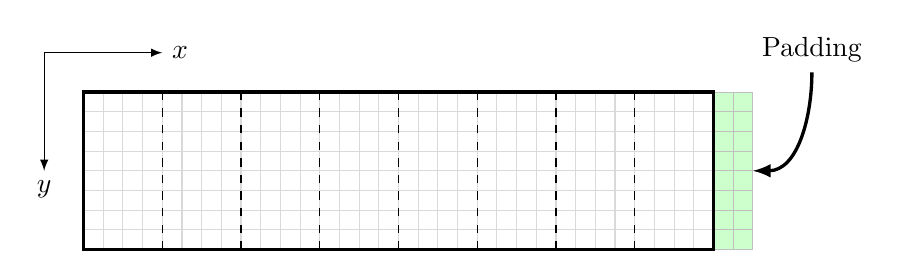
\begin{tikzpicture}[x=0.5cm,y=0.5cm]

\fill[green!20] (16,0) rectangle (17,4);
\draw[gray!30!white,step=0.5] (0,0) grid (16,4);
\draw[gray!50!white,step=0.5] (16,0) grid (17,4);
\draw[dashed,xstep=16/8,ystep=4] (0,0) grid (16,4);
\draw[very thick] (0,0) rectangle (16,4);

\coordinate (pad) at (17, 2);
\draw[-latex,very thick] (pad)+(1.5,+2.5) node[above] {Padding}
				to[out=-90,in=0] (pad);

\coordinate (O) at (-1, 5, 0);
\draw[-latex] (O) -- +(3, 0,  0) node [right] {$x$};
\draw[-latex] (O) -- +(0,  -3, 0) node [below] {$y$};
\end{tikzpicture}
\caption{A block divided in eight regions, each corresponding to a plasma chunk.  
Extra padding is added at the right for internal use in the FFTW library.}
\label{fig:block}
\end{figure}%}}}

A simplified representation of a block can be observed in the 
figure~\ref{fig:block}, where the X dimension of each field is contiguous in 
memory.  Notice the padding region in green, which is needed for the FFTW 
library to store intermediate values. The use of ghost elements is needed for 
communications and will be detailed in the chapter~\ref{ch:comm}. If we look at 
each cell $(x,y)$ in the block we find the four components $\rho(x,y)$, 
$\phi(x,y)$, $E_x(x,y)$ and $E_y(x,y)$.

\section{Simulation flow}

Before the main loop of the simulation begins, two previous iterations are 
required to prepare the simulation. The iteration counter is initially set to 
$-2$ to account for the extra steps.

\subsection{Allocation step}

After the creation of the $P$ MPI processes, the different structures to hold 
the data are allocated. Each process is assigned a block, with the corresponding 
fields and particles.

The fields are zeroed to begin the computation and the particles must be 
initialized following the user configuration. Each particle has an index which 
is used to let the user customize the particle attributes in case is required.  
Some initialization functions are provided, which place the particles following 
a random distribution or a specified pattern.

As the particles in a chunk are initialized, their position can set to any point 
in the physical space of the simulation, as no constraints are imposed for the 
initial placement. As a consequence, they need to be translated to the correct 
chunk before the simulation begins. We will refer to the initial movement of 
particles around the chunks as global communication, and is expected to last 
more than the typical communications once the simulation is running, as only 
local communications will be needed between neighbour chunks.

At soon as each particle is properly placed in the correct chunk, an initial 
computation of the charge density is done and the iteration counter is 
incremented.

\subsection{Rewind step}

The main loop begins with an special iteration that will only change the speed 
of the particles. The speed must be computed at half a time-step backwards in 
time, in order to use the leap-frog integrator as described in the 
section~\ref{sec:motion}. Once the iteration finishes, the main loop of can 
begin its normal execution with the iteration counter set to 0.

\subsection{Main loop}

The loop of the simulation performs four main steps:

\begin{itemize}
\item Accumulate charge density $\rho$ from the position of the particles.
\item Solve the field equation to get the electric field $\E$.
\item Interpolate the electric field $\E$ at particle positions.
\item Move the particles based on the computed force.
\end{itemize}

\section{Loop parallelization}

The four main steps of the simulation loop are parallelized following a common 
scheme: the block is partitioned in the same regions as the plasma chunks, which 
are processed in parallel.

\subsection{Charge accumulation}

%\begin{figure}[ht]%{{{
\begin{wrapfigure}{O}[2.7cm]{0.15\textwidth}
\centering
\begin{tikzpicture}[scale=0.85]
\begin{scope}[
		x=1cm,
		y=1cm,
		yshift=0,
		every node/.append style={
			yslant=0.5,xslant=-1},
		yslant=0.5,
		xslant=-1
	]
	\def\dx{0.0};
	% opacity to prevent graphical interference
	\draw[step=1.5/8, black!20!white, thin] (0,0-\dx) grid (6/4,6/8+\dx);
	%defining grids
	%\draw[step=1.5, black] (0,0) grid (6,6);
	\draw[xstep=1.5, ystep=0, black, very thick] (0,0-\dx) grid
		(6/4,6/8+\dx);
	\draw[dashed, xstep=6, ystep=1.5/2, black] (0,0) grid (6/4,6/8);

	\coordinate (b) at (1.5/2, 0.75/2);

\end{scope}
\begin{scope}[
		x=1cm,
		y=1cm,
		yshift=50,
		every node/.append style={
			yslant=0.5,xslant=-1},
		yslant=0.5,
		xslant=-1
	]
	\coordinate (c) at (1.5/2, 0.75/2);

	%\fill[fill=white,fill opacity=1.0] (0,0) rectangle (6,6);
	\begin{axis}[width=3cm,height=2.35cm,
						axis lines=none,
						%hide axis,
						xmin=-1, xmax=1,
						ymin=-1, ymax=1,
						inner frame sep=0,
				]
	\addplot [blue!60!white, only marks,
		mark=*, samples=12, mark size=0.75] (rand, rand);
	\addplot [red!60!white, only marks,
		mark=*, samples=12, mark size=0.75] (rand, rand);
	\end{axis}
	%\draw[step=1.5, black, thick] (0,0) grid (6,6);
	\draw[xstep=1.5, ystep=1.5/2, black!70!white, thick] (0,0) grid (6/4,6/8);
	%\draw[dashed,xstep=6, ystep=1.5, black, thick] (0,0) grid (6,6);


	\coordinate (O) at (1.5+0.5, 0.75+0.5);
\end{scope}

%\draw[-latex,very thick] (c)+(1,2) node[above]{Plasma chunk}
%				to[out=-90,in=90] (c);
%\draw[-latex,very thick,shorten >=3pt] (b)+(-1.5,-1) node[below]{Block}
%				to[out=90,in=180+45] (b);
\draw[-latex,ultra thick,shorten <=0.5cm]
	(c) to[out=-90,in=90] (b);
%	(c) to[out=-90,in=90]  node[midway,right]{Interpolation} (b);

\begin{scope}[
		y={(-1cm,0.5cm)},x={(1cm,0.5cm)}, z={(0cm,1cm)},
	]
%	\coordinate (O) at (-3, 3.5, 0);
%	\draw[-latex] (O) -- +(1, 0,  0) node [right] {$x$};
%	\draw[-latex] (O) -- +(0, -1, 0) node [right] {$y$};
%	\coordinate (O) at (-0.75, -0.75, 0);
%	\draw[-latex] (O) -- +(-1, 0,  0) node [left] {$y$};
%	\draw[-latex] (O) -- +(0, -1, 0) node [right] {$x$};
\end{scope}
\end{tikzpicture}
%\caption{Interpolation of the electric field $\E$ to the particles in a chunk.}
%\label{fig:interpolation-E}
\end{wrapfigure}
%\end{figure}%}}}
%
The interpolation process described in the equation~\ref{eq:charge-accumulation} 
is executed in parallel for all the particles of each chunk. The charge density 
field is being updated in parallel, which involves the four surrounding grid 
points of a particle, and it may happen that at the frontier of two chunks a 
concurrent access to the same element occurs.

To avoid a race condition with the next chunk, a dependency is added with the 
directive \texttt{commutative}, which allows the execution of the tasks in any 
order, but guarantees that a chunk can only be acessed by one task at a time. A 
detailed discussion on the directive can be found in the 
section~\ref{sec:exchange-x} with other alternatives to avoid a chain of 
dependencies in the case \texttt{inout} was used.

\begin{figure}[h]
\begin{lstlisting}[caption={Task to update $\rho$ field using the 
\texttt{commutative} directive}, captionpos=b]
for (i=0; i<plasma->nchunks; i++)
{
	c0 = &plasma->chunks[i];
	c1 = &plasma->chunks[(i + 1) % plasma->nchunks];
	#pragma oss task commutative(*c0, *c1) label(rho_update_0)
	rho_update(sim, i);
}
\end{lstlisting}
\end{figure}
% XXX Notice that we cannot have commutative in the next step or in the previous
% otherwise we can get ot of order execution in a chunk.

\subsection{Solve the fields}

Once the charge density is accumulated for each chunk, the electric potential 
can be computed by solving the Poisson equation (Eq.~\ref{eq:poisson}).  Using 
the MFT solver requires the computation of the Fourier transform of the charge 
density field, which has been purposely distributed among the Y dimension into 
blocks: The computation of the FFT can then be distributed into each process.

To parallelize the execution in each process, two mechanism are available in the 
FFTW library: pthreads and OpenMP. The multithreading design is based on the 
model of the \textit{parallel for}, where the total number of iterations are 
divided into parts that can be executed in parallel.
%
\begin{figure}[ht]%{{{
\begin{lstlisting}[
	%float,
	label={lst:openmp-for},
	caption={Parallel for with OpenMP used in the FFTW library.}]
#pragma omp parallel for private(d)
for (i = 0; i < nthr; ++i) {
	...
	proc(&d);
}
\end{lstlisting}
\end{figure}%}}}
%
In the listing~\ref{lst:openmp-for} the OpenMP parallelization method is shown, 
as used in the FFTW. With minor changes we can adapt the model to OmpSs-2, 
following the same approach. A task is created for each iteration and then we 
wait for the completion of all of them, ensuring all iterations of the loop have 
been executed, as can be seen in the listing~\ref{lst:ompss-for}. A comparative 
analysis of the different methods is provided in the chapter~\ref{ch:analysis}.
%
\begin{figure}[ht]%{{{
\begin{lstlisting}[
	%float,
	label={lst:ompss-for},
	caption={Parallel for with OmpSs-2 using tasks.}]
for (i = 0; i < nthr; ++i) {
	#pragma oss task private(d)
	{
		...
		proc(&d);
	}
}
#pragma oss taskwait
\end{lstlisting}
\end{figure}%}}}
%

Once we obtain the electric potential $\phi$ after the MFT algorithm, we can 
compute the electric field $\E$ in both directions $E_x$ and $E_y$. The 
operation can be fully parallelized in tasks by the division of the block in the 
same regions as the plasma chunks. It is not necessary that the same division is 
used, but has the advantage of simplify how the dependencies between plasma and 
fields are written.
%
\begin{figure}[ht]%{{{
\begin{lstlisting}[
label={lst:compute-E},
caption={Computation of E in parallel by chunks.}]
for(ic=0; ic<sim->plasma.nchunks; ic++)
{
	chunk = &sim->plasma.chunks[ic];
	#pragma oss task inout(*chunk) label(field_E_compute)
	field_E_compute(sim, chunk);
}
\end{lstlisting}
\end{figure}%}}}
%
The same division provided by the plasma chunks is used as a first approximation 
as shown in the listing~\ref{lst:compute-E}, but other number of regions are 
possible.

\subsection{Field interpolation}
%
%\begin{figure}[ht]%{{{
\begin{wrapfigure}{O}[2.5cm]{0.15\textwidth}
\centering
\begin{tikzpicture}[scale=0.8]
\begin{scope}[
		x=1cm,
		y=1cm,
		yshift=0,
		every node/.append style={
			yslant=0.5,xslant=-1},
		yslant=0.5,
		xslant=-1
	]
	\def\dx{0.0};
	% opacity to prevent graphical interference
	\draw[step=1.5/8, black!20!white, thin] (0,0-\dx) grid (6/4,6/8+\dx);
	%defining grids
	%\draw[step=1.5, black] (0,0) grid (6,6);
	\draw[xstep=1.5, ystep=0, black, very thick] (0,0-\dx) grid
		(6/4,6/8+\dx);
	\draw[dashed, xstep=6, ystep=1.5/2, black] (0,0) grid (6/4,6/8);

	\coordinate (b) at (1.5/2, 0.75/2);

\end{scope}
\begin{scope}[
		x=1cm,
		y=1cm,
		yshift=50,
		every node/.append style={
			yslant=0.5,xslant=-1},
		yslant=0.5,
		xslant=-1
	]
	\coordinate (c) at (1.5/2, 0.75/2);

	%\fill[fill=white,fill opacity=1.0] (0,0) rectangle (6,6);
	\begin{axis}[width=3cm,height=2.35cm,
						axis lines=none,
						%hide axis,
						xmin=-1, xmax=1,
						ymin=-1, ymax=1,
						inner frame sep=0,
				]
	\addplot [blue!60!white, only marks,
		mark=*, samples=12, mark size=0.75] (rand, rand);
	\addplot [red!60!white, only marks,
		mark=*, samples=12, mark size=0.75] (rand, rand);
	\end{axis}
	%\draw[step=1.5, black, thick] (0,0) grid (6,6);
	\draw[xstep=1.5, ystep=1.5/2, black!70!white, thick] (0,0) grid (6/4,6/8);
	%\draw[dashed,xstep=6, ystep=1.5, black, thick] (0,0) grid (6,6);


	\coordinate (O) at (1.5+0.5, 0.75+0.5);
\end{scope}

%\draw[-latex,very thick] (c)+(1,2) node[above]{Plasma chunk}
%				to[out=-90,in=90] (c);
%\draw[-latex,very thick,shorten >=3pt] (b)+(-1.5,-1) node[below]{Block}
%				to[out=90,in=180+45] (b);
\draw[-latex,ultra thick,shorten >=0.5cm]
	(b) to[out=90,in=-90] (c);
%	(b) to[out=90,in=-90]  node[midway,right]{Interpolation} (c);

\begin{scope}[
		y={(-1cm,0.5cm)},x={(1cm,0.5cm)}, z={(0cm,1cm)},
	]
%	\coordinate (O) at (-3, 3.5, 0);
%	\draw[-latex] (O) -- +(1, 0,  0) node [right] {$x$};
%	\draw[-latex] (O) -- +(0, -1, 0) node [right] {$y$};
%	\coordinate (O) at (-0.75, -0.75, 0);
%	\draw[-latex] (O) -- +(-1, 0,  0) node [left] {$y$};
%	\draw[-latex] (O) -- +(0, -1, 0) node [right] {$x$};
\end{scope}
\end{tikzpicture}
%\caption{Interpolation of the electric field $\E$ to the particles in a chunk.}
%\label{fig:interpolation-E}
\end{wrapfigure}
%\end{figure}%}}}
%
Once the electric field of a chunk is ready, the value is interpolated at the 
particle locations. The force will be obtained in the next step from the 
interpolated electric field in each particle.

Each chunk can be processed independently by one task, but a \texttt{inout} 
dependency must be added to ensure the order of execution of a chunk is done 
after the electric field is computed, as observed in the 
listing~\ref{lst:interpolate-E}.
%
\begin{figure}[ht]%{{{
\begin{lstlisting}[
label={lst:interpolate-E},
caption={Interpolation of the electric field $\E$ at particle position.}]
for(i=0; i<sim->plasma.nchunks; i++)
{
	chunk = &sim->plasma.chunks[i];
	#pragma oss task inout(*chunk) label(chunk_E)
	{
		for(is=0; is<chunk->nspecies; is++)
		{
			particle_set_E(sim, chunk, is);
		}
	}
}
\end{lstlisting}
\end{figure}%}}}
%
\subsection{Particle mover}

The force acting on each particle is obtained as described in the 
equation~\ref{eq:force}, as the combination of the electric and magnetic forces.  
The electric term is computed from the interpolated electric field at the 
particle locations and each chunk can begin the process as soon as the 
interpolation process has finished.

A task is created for each chunk, and the particles are moved accordingly to the 
obtained force. The Boris integrator described in the section~\ref{sec:boris} is 
used to accurately position the particles. An \texttt{inout} dependency is added 
to each chunk to guarantee the order of execution: after the electric field is 
interpolated in the particles, as shown in the listing~\ref{lst:particle-mover}.
%
\begin{figure}[ht]%{{{
\begin{lstlisting}[
label={lst:interpolate-E},
caption={Interpolation of the electric field $\E$ at particle position.}]
for(i=0; i<sim->plasma.nchunks; i++)
{
	chunk = &sim->plasma.chunks[i];
	#pragma oss task inout(*chunk) label(chunk_x_update)
	{
		for(is=0; is<chunk->nspecies; is++)
		{
			particle_x_update(sim, chunk, is);
		}
	}
}
\end{lstlisting}
\end{figure}%}}}
